\myparagraph{Purpose}
As we have the possibilty in \textit{Track4Run} for an organizer to create a new \textit{Run}, the system must also be able to manage the decision of an organizer to delete a \textit{Run}.

\myparagraph{Scenario}
Alice wants to delete a \textit{Run} that she had organized for the next month, because the weather forecast are not optimal.
In order to avoid a rainy day Alice opened \textit{Track4Run} web-site, she logged in and she clicked on the "\textit{Manage a Run}" button.
On top of the table there was the \textit{Run} that she was looking for and she clicked on its "\textit{Delete}" button.
After that a mail arrived in Alice mailbox, it was the confirmation of the elimination of the \textit{Run}.

\myparagraph{Use Case}
The \textit{Delete A Run} use case is analyzed in Table \ref{table:deleteRunTable}.

\myparagraph{Functional requirements}
\begin{enumerate}
  \item The system must not show \textit{Run}, in \textit{Manage a Run} section, of which an \textbf{Organizer} is not the owner;
  \item The system must let the \textbf{Organizer} leave the deletion process at anytime.
\end{enumerate}

\begin{center}
\begin{table}
\begin{tabular}{ | l | p{0.75\linewidth} | }
  \hline
    Actor & \textbf{Organizer} \\ \hline
    Goal & \textbf{[G.11]} \\ \hline
    Input Condition & An \textbf{Organizer} wants to delete a \textit{Run} \\ \hline
    Event Flow & \begin{minipage}[t]{0.7\textwidth}
      \begin{enumerate}
        \item The \textbf{Organizer} opens \textit{Track4Run} service through web application and he/she logs in;
        \item The \textbf{Organizer} clicks on the "\textit{Manage a Run}" button;
        \item The \textbf{Organizer} looks for a \textit{Run} through the search bar or looking to the proposed ones;
        \item The \textbf{Organizer} clicks on the "\textit{Delete}" button of the targeted \textit{Run}.
      \end{enumerate}
    \smallskip
  \end{minipage} \\ \hline
  Output Condition & The system deletes the \textit{Run} and notifies the \textbf{Organizer} with a confirmation e-mail. Moreover the system must notify all enrolled people in the \textit{Run} with a e-mail and delete their enrolments. \\ \hline
  Exceptions & \begin{minipage}[t]{0.7\textwidth}
    \begin{itemize}
      \smallskip
      \item If the \textbf{Organizer} looks for a \textit{Run} that is not present in the system or he/she is not the owner, the system notifies the \textbf{Organizer} with a warning message;
      \item If the \textbf{Organizer} decides to leave the elimination process this one is aborted.
    \end{itemize}
    \smallskip
  \end{minipage}  \\ \hline
\end{tabular}
\caption{\textit{Delete A Run} use case}
\label{table:deleteRunTable}
\end{table}
\end{center}

\begin{figure}
\begin{center}
  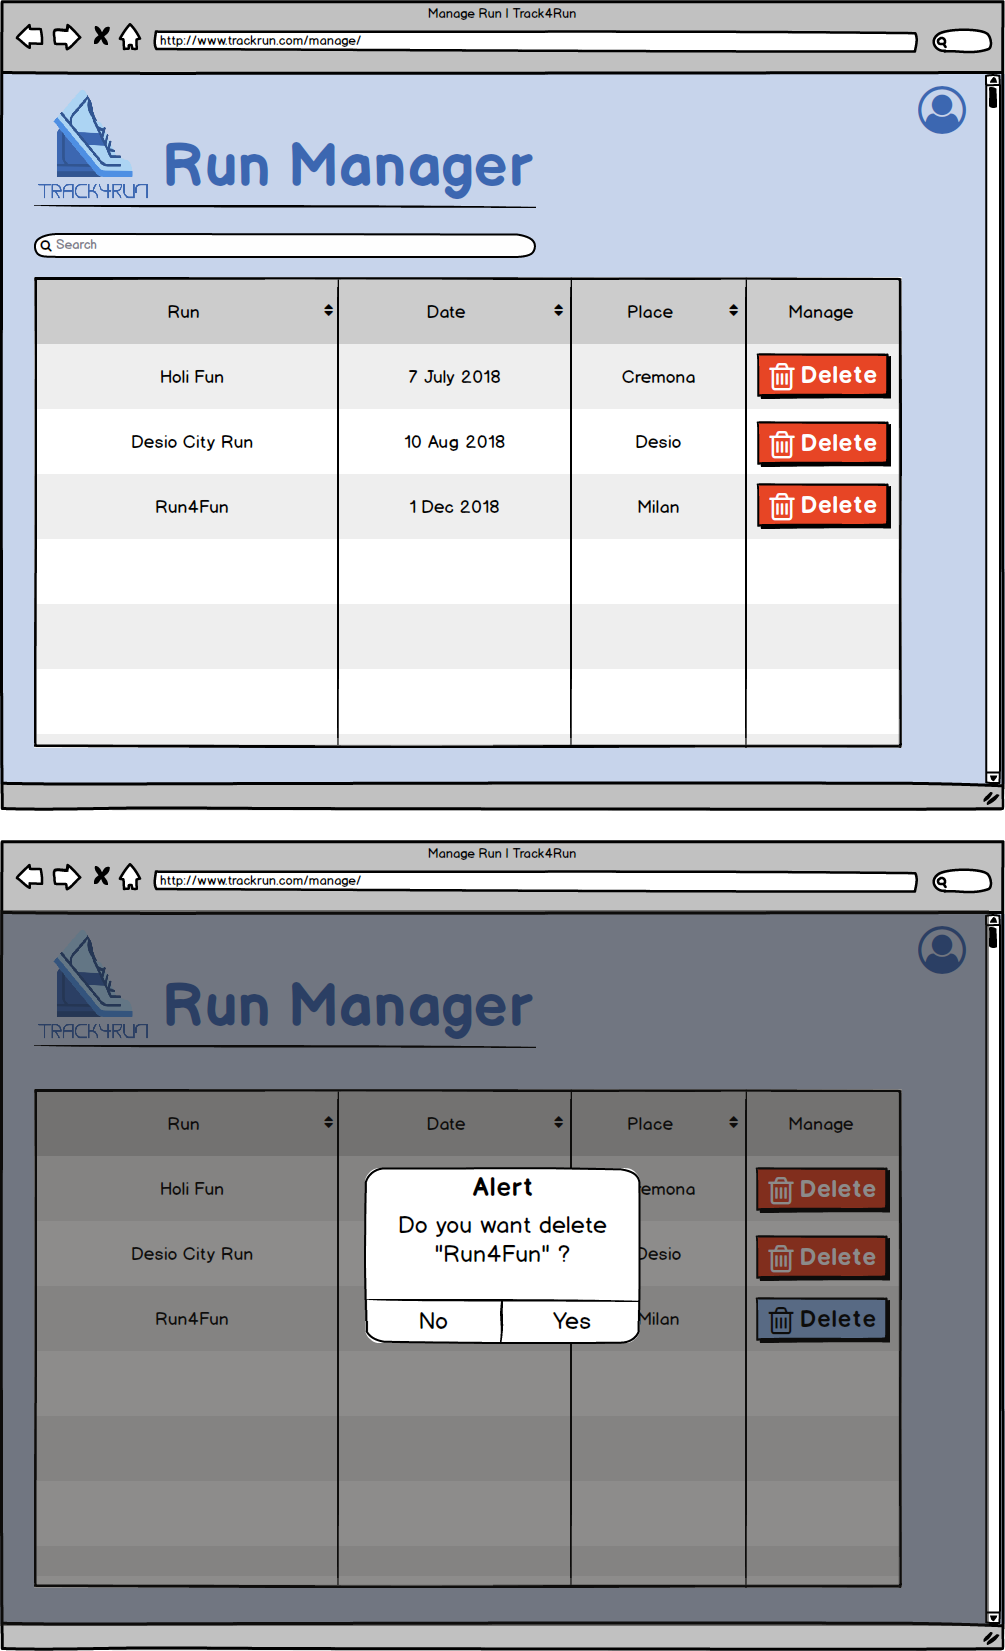
\includegraphics[width=\textwidth]{img/mockup/DeleteRun.png}
  \hspace{0.05\linewidth}
  \centering
  \caption{\textit{Delete A Run} mockup}
  \label{img:deleteRunMockup}
\end{center}
\end{figure}
